\chapter{Results and discussion}
To see which feature size each algorithm performed best with we messured in-domain sentimental analysis on all algorithm with 11 pre-selected different feature vectors as input data. The result in presented in Figure ~\ref{fig:featuresize}. In the Figure each line corresponds to an algorithm and the bars represent one standard deviation (??). KNN has better performance with a lower feature size whilst the rest has better performance with a large feature size. This result was expected. 
\begin{figure}[h!]
\centering
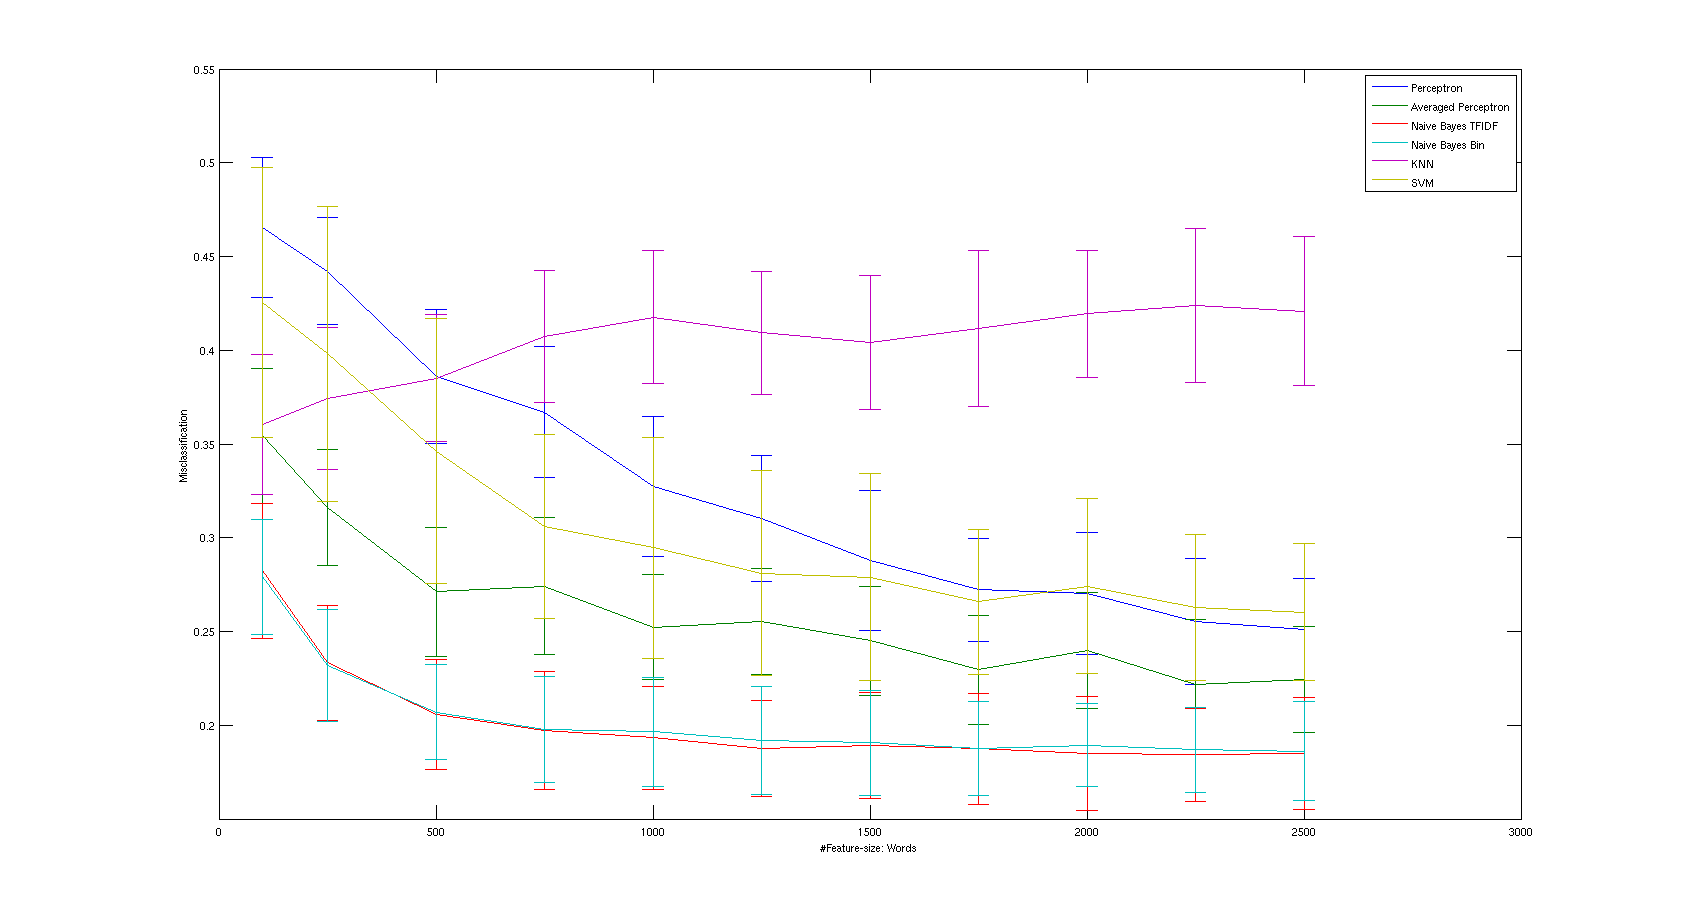
\includegraphics[scale = 0.2]{fig/featuresize_plot_snowball_unigram.png}
\caption{In-domain classification of different feature size with stddeviation and all algorithms.}
\label{fig:featuresize}
\end{figure} \\\\
We continued with each algorithms best feature size and messured how the training-set size would affect the classification. The result is found in \ref{fig:trainingsize} where each algorithm is represented by a line and the x-axis consists of different percentages of the total training size. 
\begin{figure}[h!]
\centering
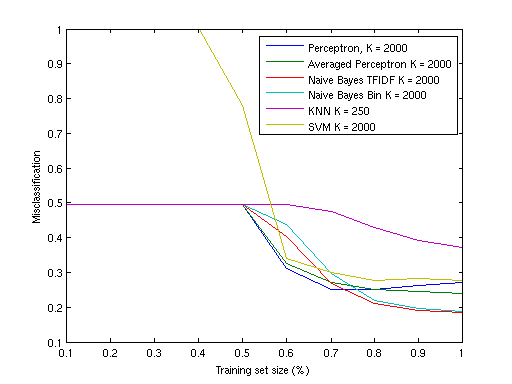
\includegraphics[scale = 0.5]{fig/training-size.png}
\caption{All algorithms with different training set size}
\label{fig:trainingsize}
\end{figure}  \\\\
The SVM-algorithm is not converging until around $~40 \%$ and this is the reason why it has $100 \%$ misclassification. With small training size the algorithms perform slightly better than random assignment, $50 \%$, but the bigger training size the better result. Naive Bayes is the algorithm with best performance whilst the two Perceptron and SVM has almost equal performance. 
\\\\
%How does it fare against your benchmarks and instances? Describe advantages and disadvantages, possibly in relation to other groups in this course.
%* bättre eller sämre reslutat än förväntat? varför?
%* jämför algoritmerna, hur bra är de? hur lång tid tar de?\\
\section{Text categorization}
Här skriver vi om vad vi fick för resultat
\section{Out-of-domain}
Här skriver vi om vad out of domain gav
\section{Correlation Text categorization and Out-of-domain}
Skriva om correlationen
%text categorization:\\
%* plot över de olika algorithmerna och hur bra de kategoriserar. (en plot med alla?)

\section{Discussion}

